\documentclass[10pt]{article}
\textwidth 6.5in
\textheight 9in
\oddsidemargin -0.2in
\topmargin -0.5in

\usepackage{graphicx,times,amsmath} % Add all your packages here
\usepackage[all]{xy}
\usepackage{multirow}
\usepackage{graphicx}
\usepackage{color}
\usepackage{tabularx}
\usepackage{url}
\usepackage{amsmath}
\usepackage{amssymb}
\usepackage[noend,ruled,linesnumbered]{algorithm2e}

\newenvironment{program*}[1][htb]
  {\renewcommand{\algorithmcfname}{Program}% Update algorithm name
   \begin{algorithm*}[#1]%
  }{\end{algorithm*}}

\usepackage[numbers, sort]{natbib}

\usepackage{listings}
\usepackage[svgnames]{xcolor}
%\usepackage{newtxtext}
\definecolor{javared}{rgb}{1,0,0} % for strings
\definecolor{javagreen}{rgb}{0.25,0.5,0.35} % comments
\definecolor{javapurple}{rgb}{0.5,0,0.35} % keywords
\definecolor{javadocblue}{rgb}{0.25,0.35,1} % javadoc
\lstset{language=Java,
keywordstyle=\color{javapurple}\bfseries,
  stringstyle=\color{javared},
  commentstyle=\color{javagreen},
  basicstyle=\tt\footnotesize,        % the size of the fonts that are used for the code
  breakatwhitespace=false,         % sets if automatic breaks should only happen at whitespace
  breaklines=true,                 % sets automatic line breaking                   % sets the caption-position to bottom
  extendedchars=true,              % lets you use non-ASCII characters; for 8-bits encodings only, does not work with UTF-8
  showspaces=false,                % show spaces everywhere adding particular underscores; it overrides 'showstringspaces'
  showstringspaces=false,          % underline spaces within strings only
  showtabs=false,                  % show tabs within strings adding particular underscores
  tabsize=2,                     % sets default tabsize to 2 spaces
  numbers=left,
  }
\lstdefinestyle{highlight} {
moredelim=[is][\bfseries\textcolor{javadocblue}]{<<>>}{>><<},
moredelim=[is][\itshape]{!!}{??}
}

\begin{document}
%\graphicspath{{/Users/zhangz/research/top/presentation/figures/}}
%em is the width of a M in the current font
  %sets indentation
  \setlength{\parindent}{1em}
  %sets space between paragraphs
  \setlength{\parskip}{0em}
  %sets space between items in a list (i.e. itemize,enumerate,description)
  \setlength{\parsep}{0em}

\noindent In this tutorial, we describe steps for setting up a Maven
project that uses {\tt libSBOLj} in Eclipse, and explain how we use SBOL
2.0 to represent the function of a state-of-the-art design, namely a
CRISPR-based repression module Kiani~\textit{et
  al.}~\cite{kiani2014crispr}. 

\section*{Set up Maven plugins in Eclipse}
In this section, we describe steps for installing Maven plugins in Eclipse. The Eclipse version used is Luna Service Release 2 (4.4.2). Here are the steps:
\begin{enumerate}
\item In Eclipse, go to Help and select Install New Software, 
\item Add a new software site: Name = slf4j, URL = \url{http://www.fuin.org/p2-repository/}, 
\item Select this site to work with, expand Maven osgi-bundles, and select slf4j.api, 
\item Click Next and follow the installation process, 
\item Add a new software site: Name = Maven Plugins, URL = \url{http://download.eclipse.org/technology/m2e/releases}, 
\item Select this site to work with, expand Maven Integration for Eclipse, and select m2e - Maven Integration for Eclipse, and
\item Click Next and follow the installation process.
\end{enumerate}

\section*{Creating a new project}
After the Maven plugin is installed, we are now ready to create a new Maven project in Eclipse. The following text describe the necessary steps. 

In the package explorer window, right click and select {\bf New $\rightarrow$ Other}.
\begin{center}
  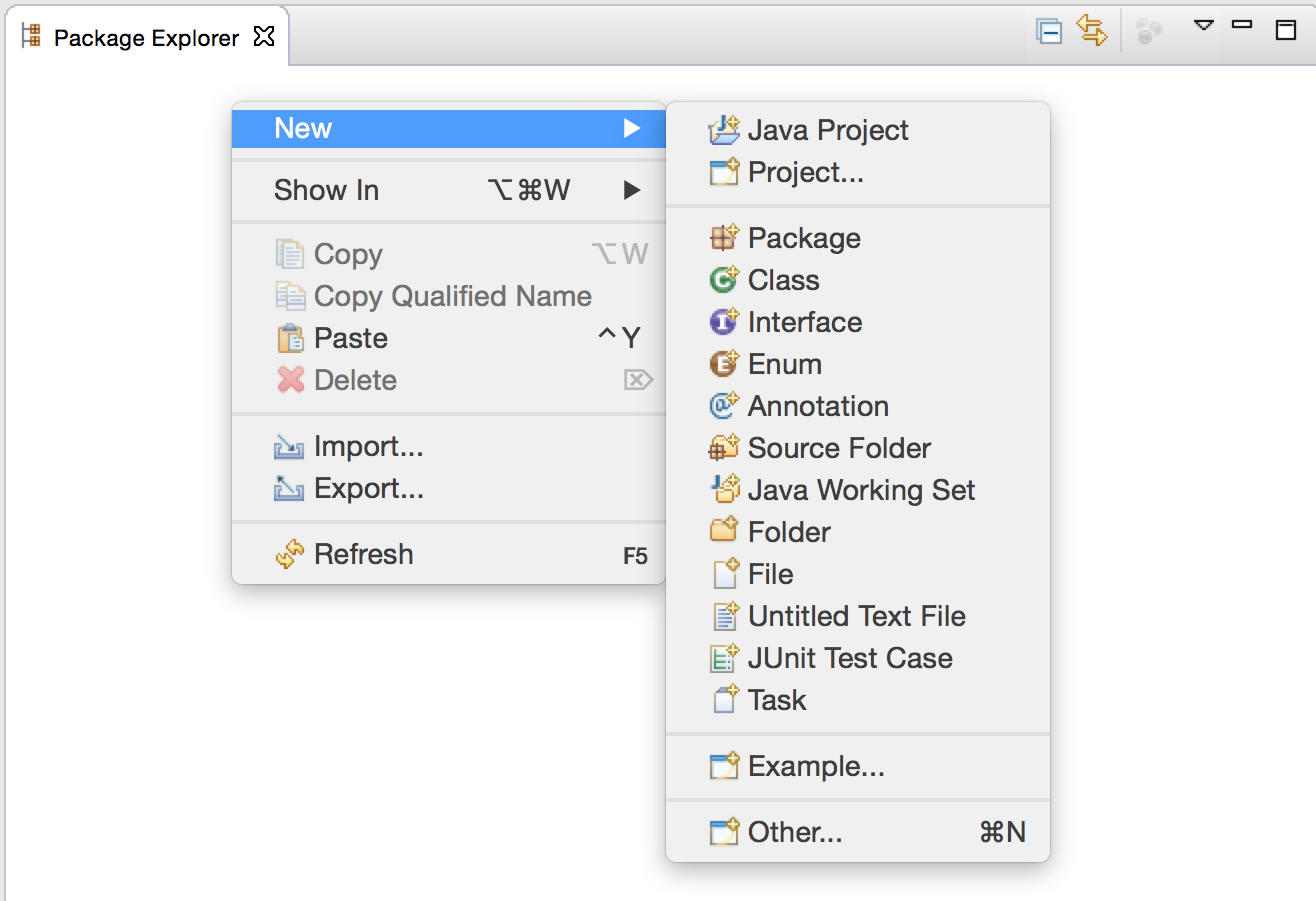
\includegraphics[width=0.8\textwidth]{figures/createNewMavenProject1}
\end{center}

Under the {\bf Maven} folder, choose {\bf Maven Project}, and then follow the default options for the project setup.
\begin{center}
  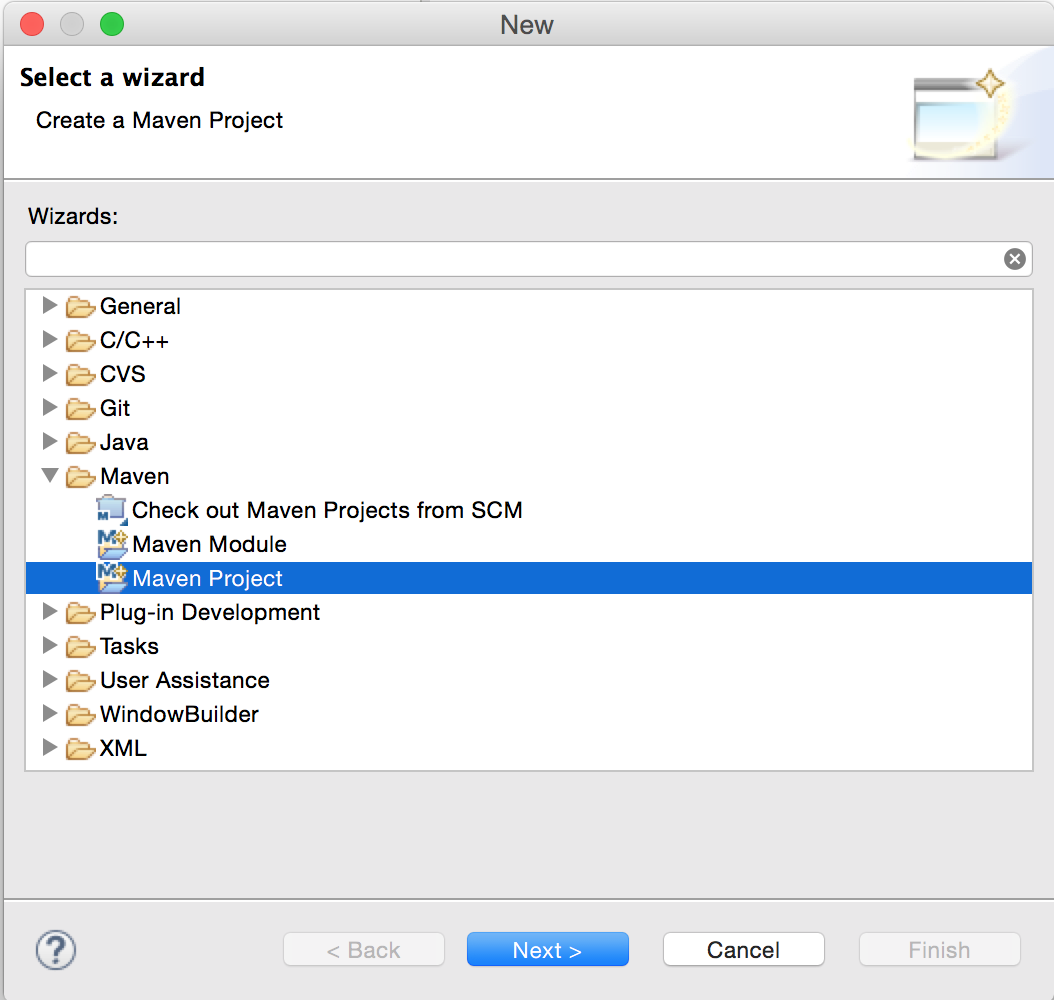
\includegraphics[width=0.75\textwidth]{figures/createNewMavenProject2}
\end{center}

% \begin{center}
%   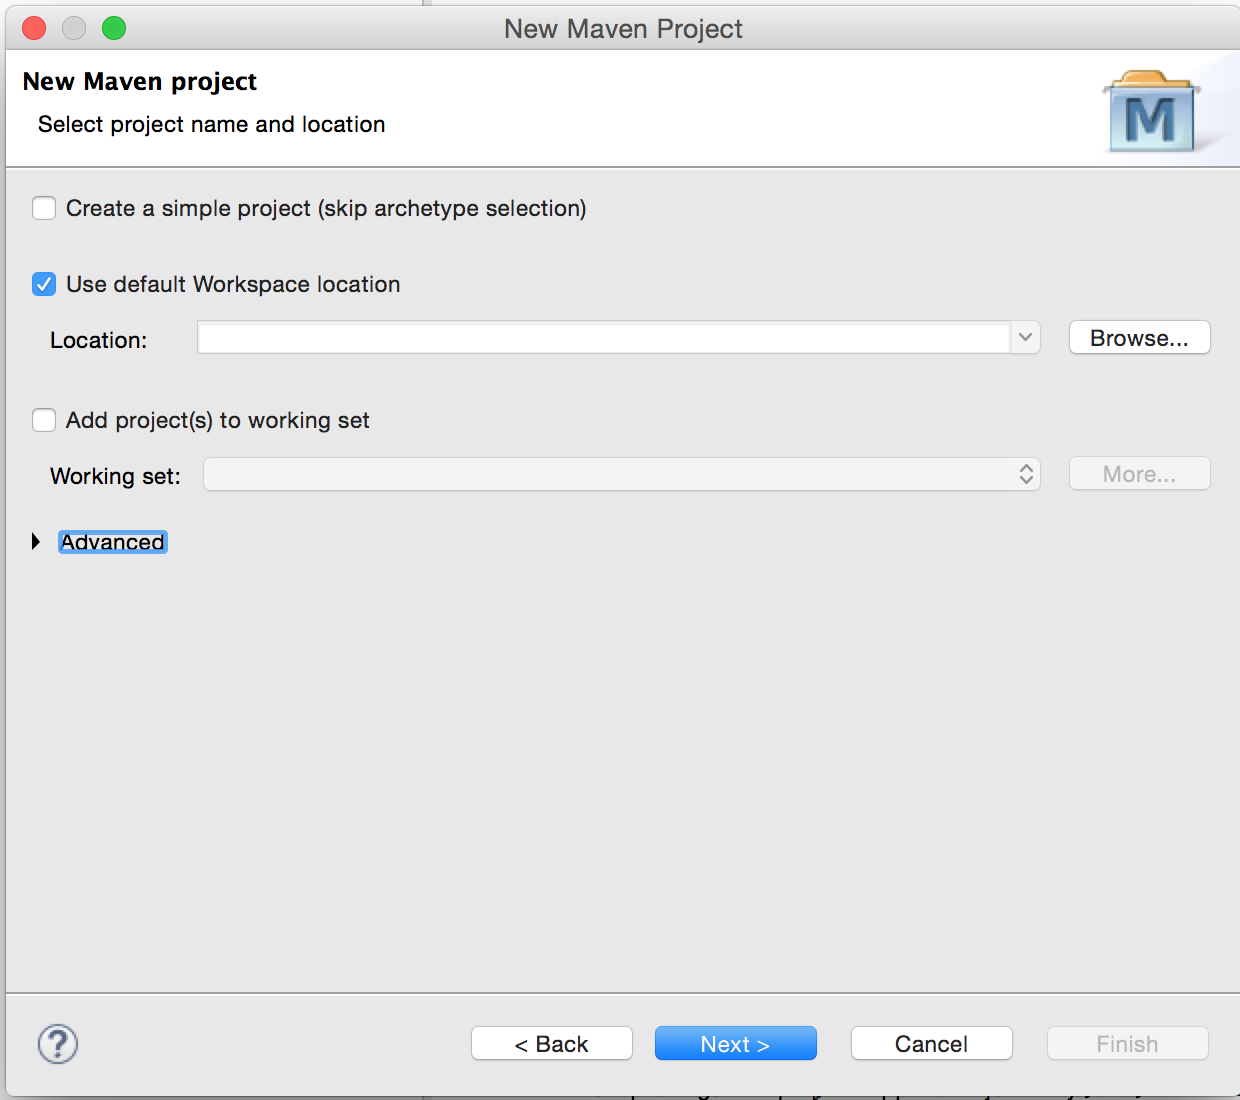
\includegraphics[width=0.8\textwidth]{figures/createNewMavenProject3}
% \end{center}

\begin{center}
  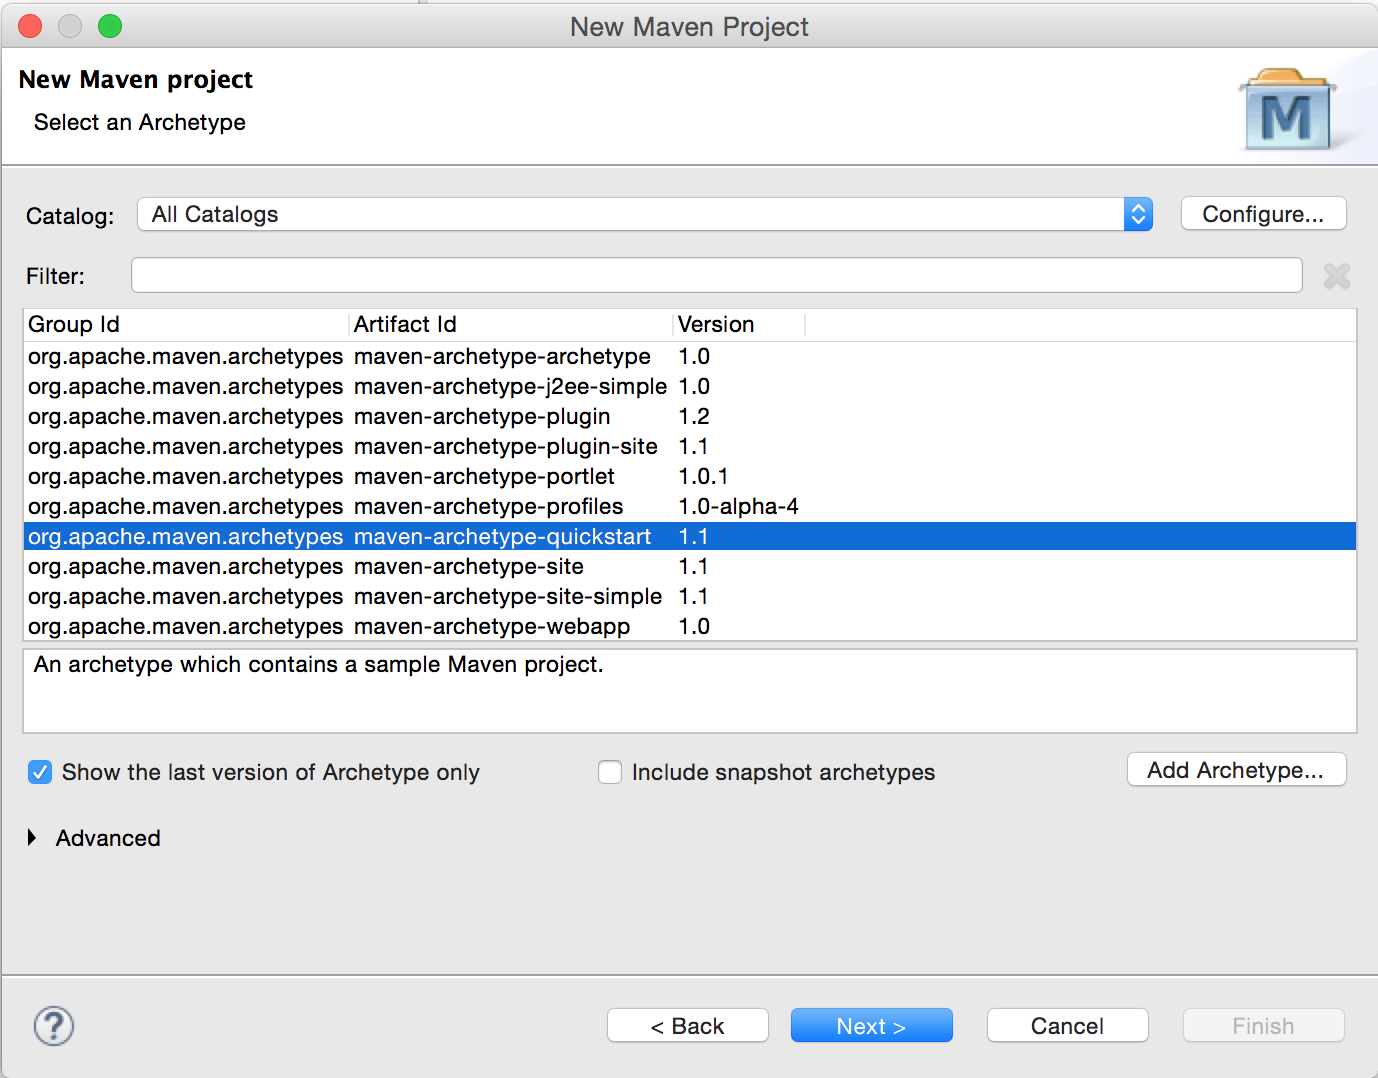
\includegraphics[width=0.75\textwidth]{figures/createNewMavenProject4}
\end{center}

In the window for specifying archetype parameters, you may type your group ID and artifact ID. In this tutorial, they are specified as shown below. 
\begin{center}
  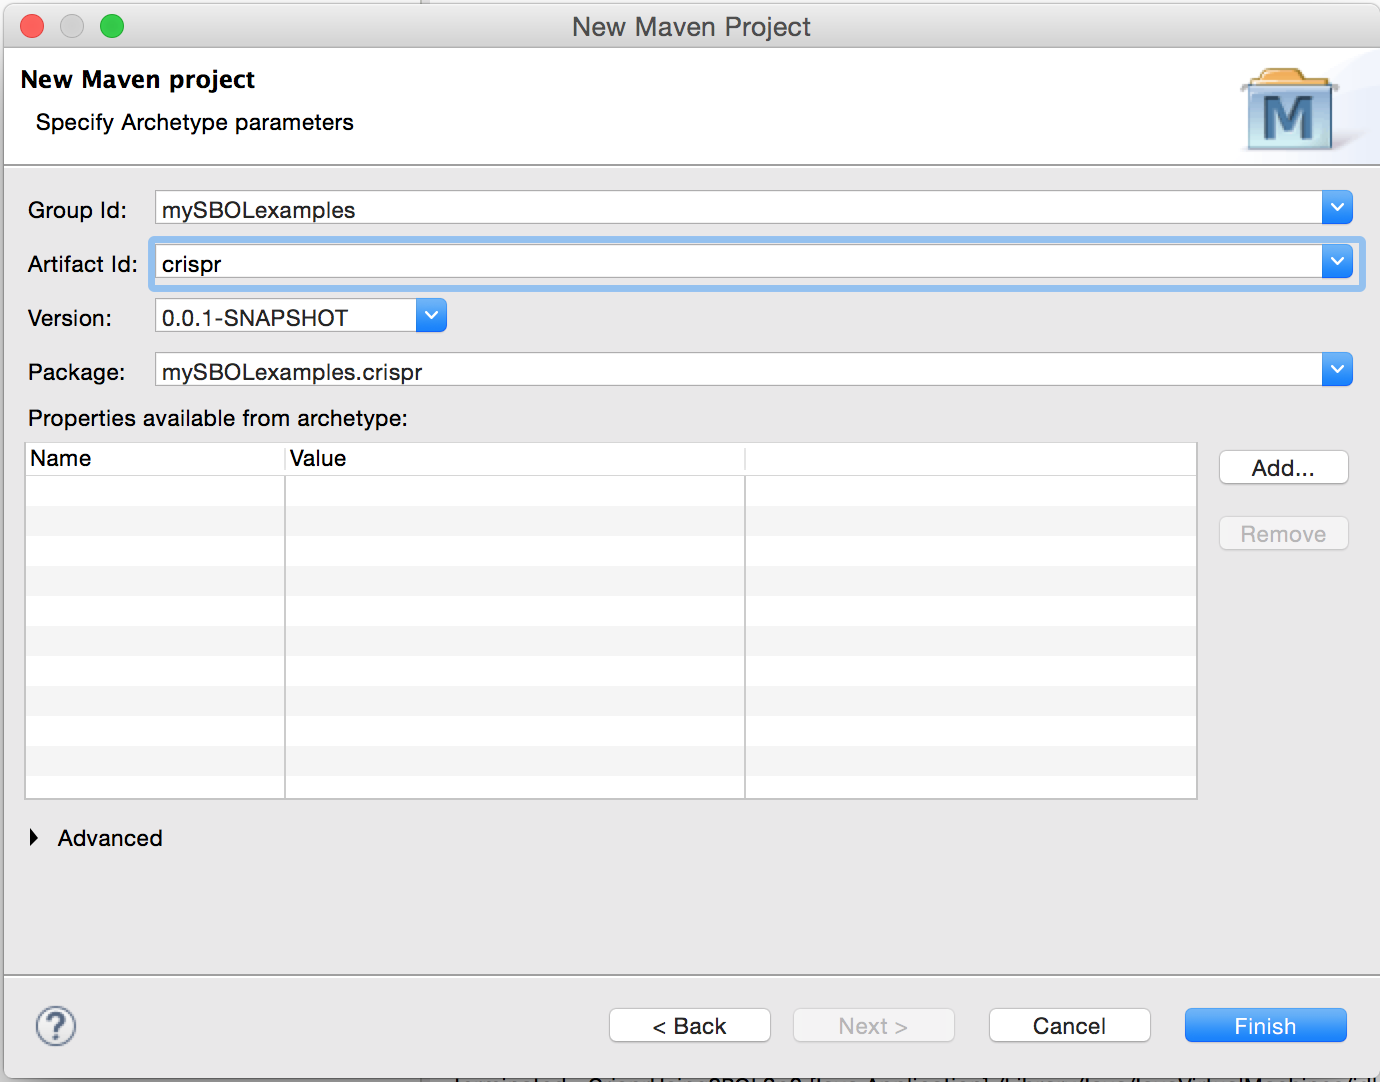
\includegraphics[width=0.8\textwidth]{figures/createNewMavenProject5}
\end{center}

Once the project setup is finished, you should be able to see two Java source folders, a {\bf JRE System Library} and a {\bf Maven Dependencies} library, and a {\bf pom.xml} file. 
\begin{center}
  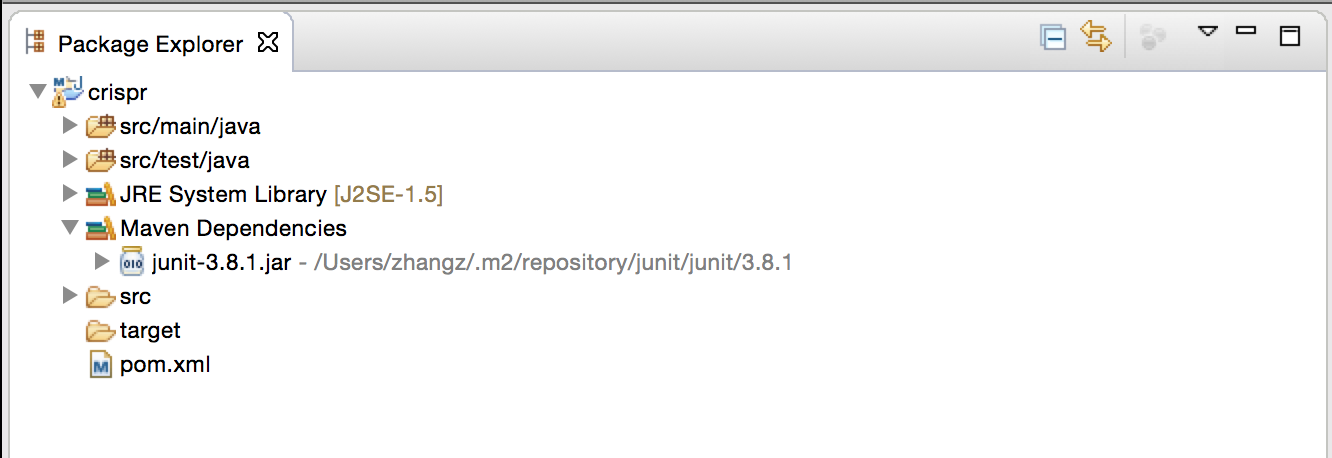
\includegraphics[width=0.8\textwidth]{figures/createNewMavenProject6}
\end{center}

It is possible that the JRE System Library created by Maven is not compatible with the installed JREs. In the screenshot shown below, it is set to {\bf J2SE-1.5}, but the Maven compiler is compatible with {\bf JavaSE-1.7} instead. To change it, right-click on JRE System Library, and select {\bf Build Path $\rightarrow$ Configure Build Path}. 
\begin{center}
  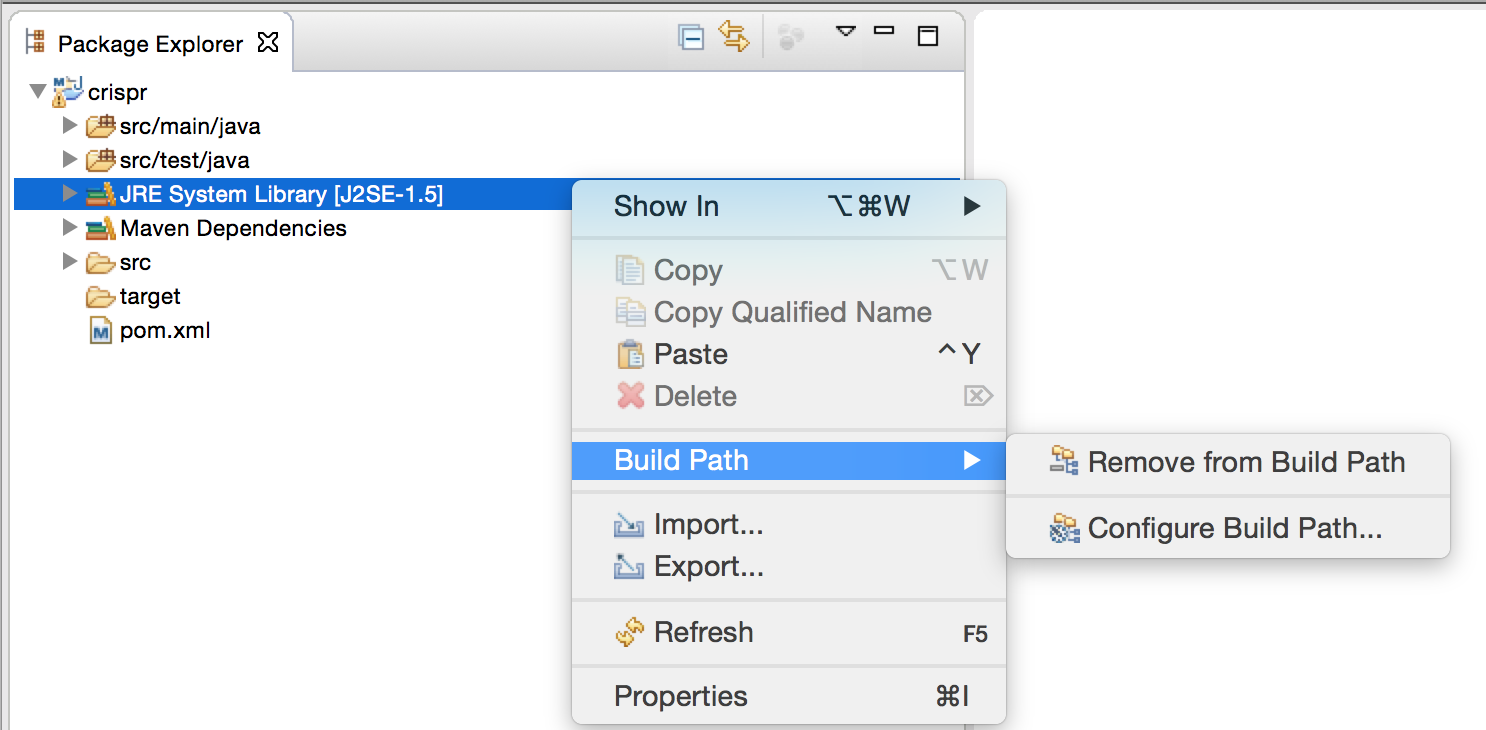
\includegraphics[width=0.8\textwidth]{figures/createNewMavenProject7}
\end{center}

In the popup properties window, select {\bf Edit} under {\bf Libraries}. 
\begin{center}
  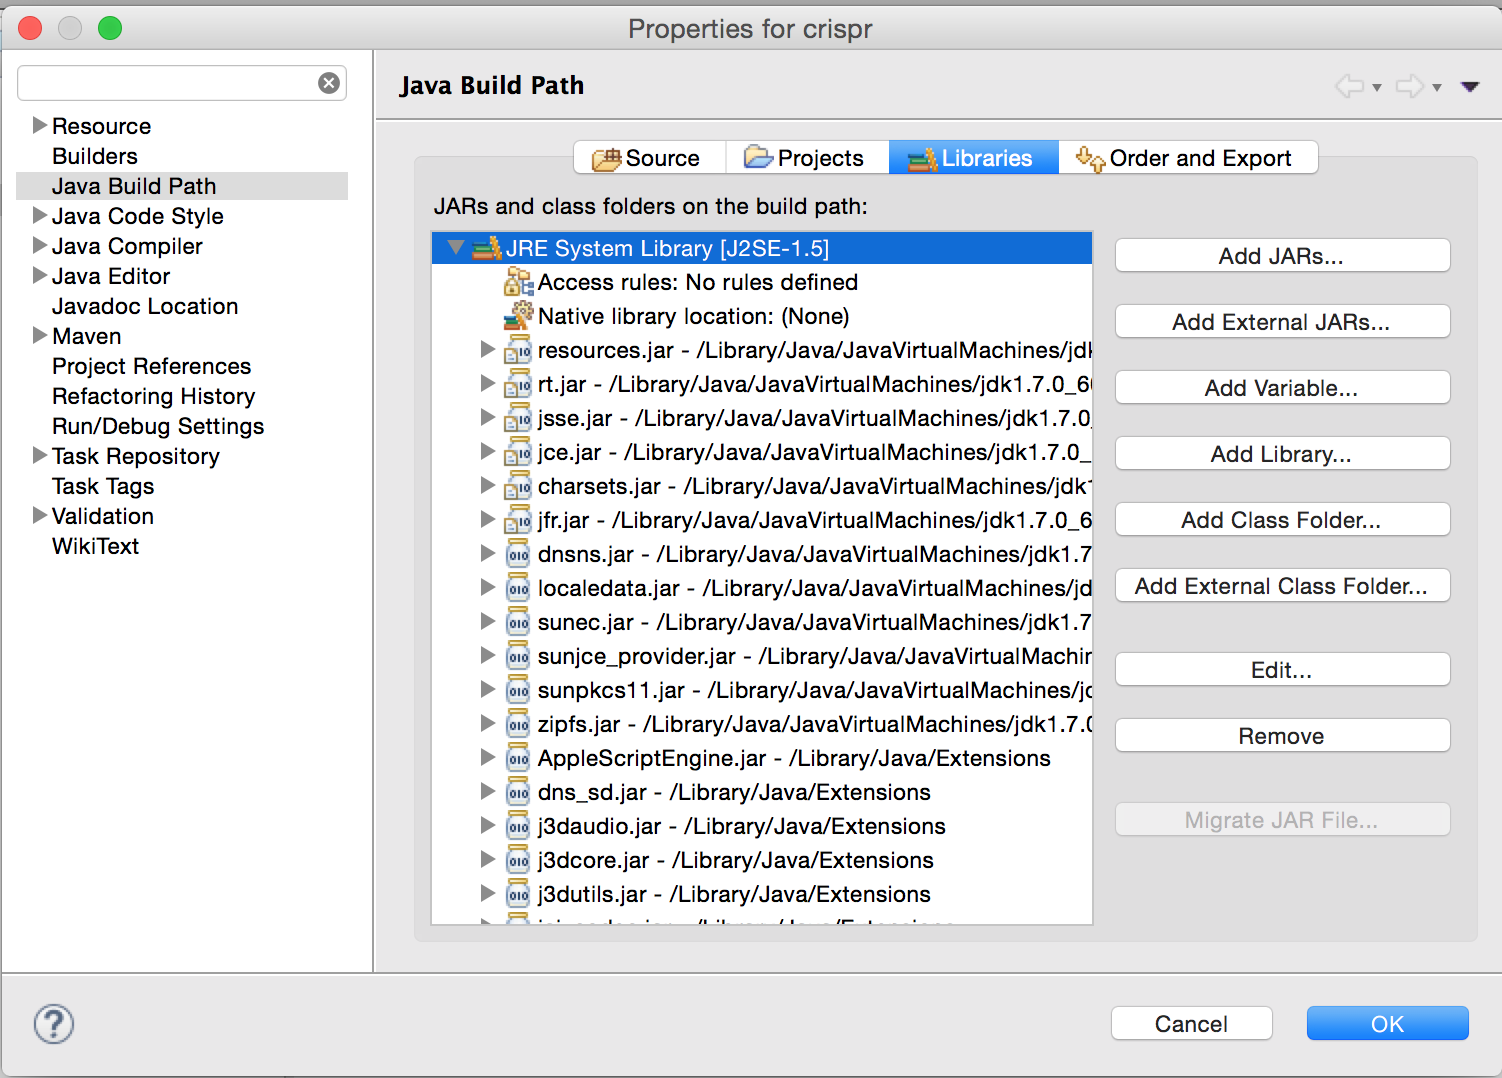
\includegraphics[width=0.8\textwidth]{figures/createNewMavenProject8}
\end{center}

We can now change the execution environment to JavaSE-1.7 as shown below. 
\begin{center}
  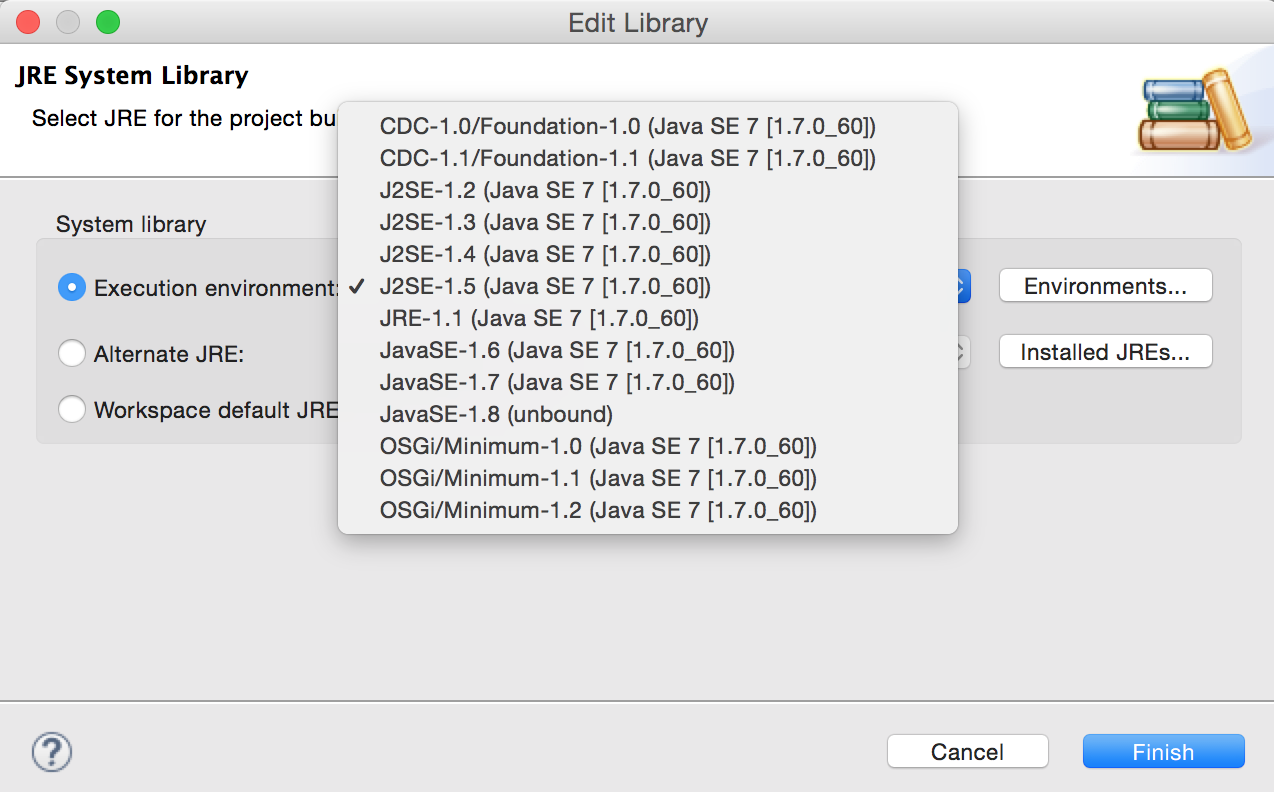
\includegraphics[width=0.8\textwidth]{figures/createNewMavenProject9}
\end{center}

This solution, however, is temporary. If we right-click on the ``crispr'' project and then select {\bf Maven $\rightarrow$  Update Project}, the JRE will reset itself back to J2SE-1.5. 
\begin{center}
  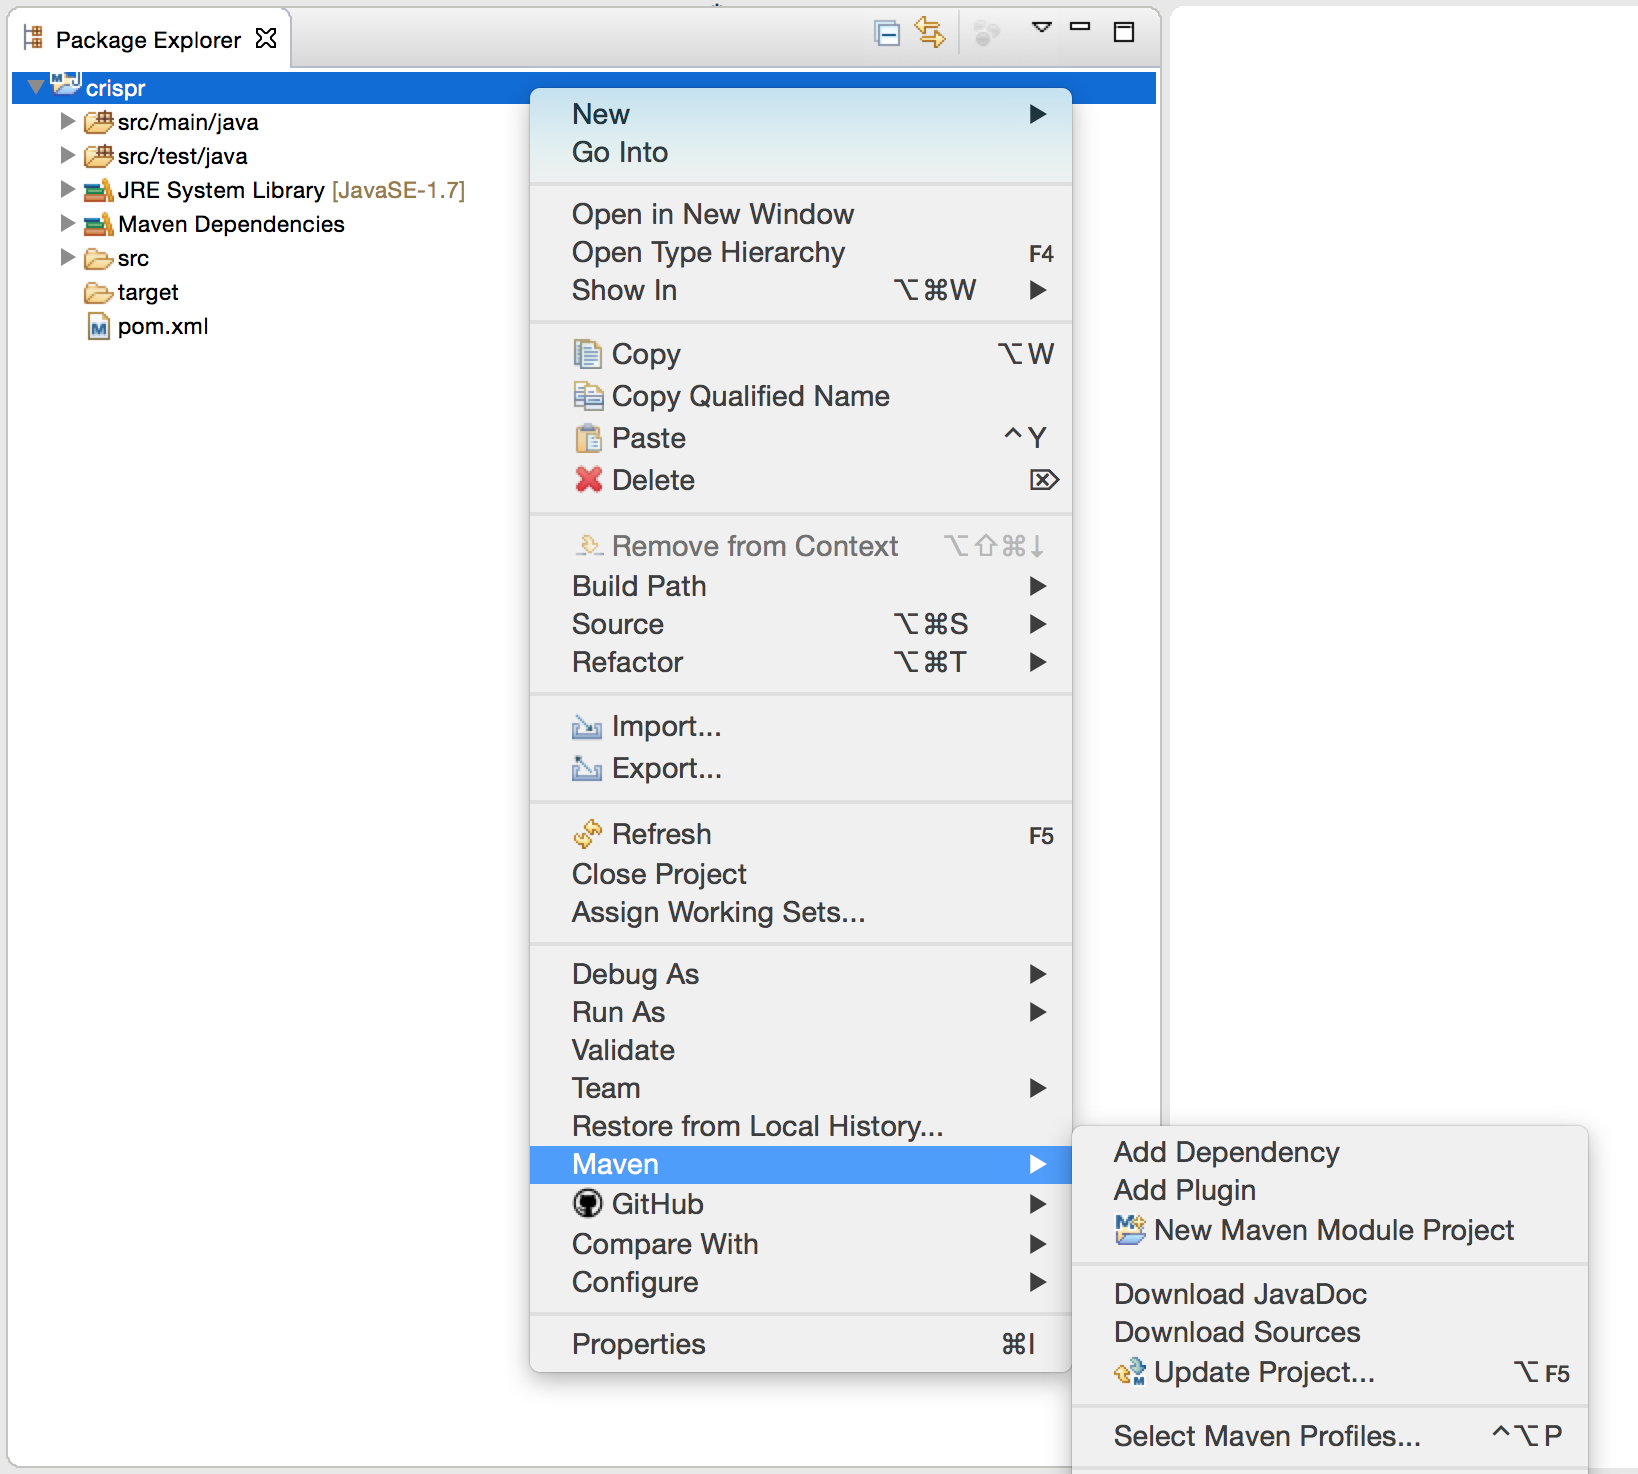
\includegraphics[width=0.8\textwidth]{figures/createNewMavenProject10}
\end{center}

A permanent fix would be to manually add the plugin management information below to the pom.xml file.

\begin{minipage}{\textwidth} 
\begin{lstlisting}[language=xml,basicstyle=\footnotesize\ttfamily]
<build>
    <pluginManagement>
        <plugins>
            <plugin>
                <groupId>org.apache.maven.plugins</groupId>
                <artifactId>maven-compiler-plugin</artifactId>
                <version>3.1</version>
                <configuration>
                    <source>1.7</source>
                    <target>1.7</target>
                </configuration>
            </plugin>
        </plugins>
    </pluginManagement>
</build>
\end{lstlisting}
\end{minipage}

The pom.xml should look like the one shown below after this modification. Remember to save the file and then do {\bf Maven $\rightarrow$  Update Project}.

\begin{minipage}{\textwidth} 
\lstinputlisting[language=xml,basicstyle=\footnotesize\ttfamily]{pom.xml}
\end{minipage}

\section*{Adding {\tt libSBOLj} as dependency}
We are now ready to add libSBOLj as a Maven dependency. This can be easily done by right-clicking on the ``crispr'' project and then select {\bf Maven $\rightarrow$ Add Dependency}.
% \begin{center}
%   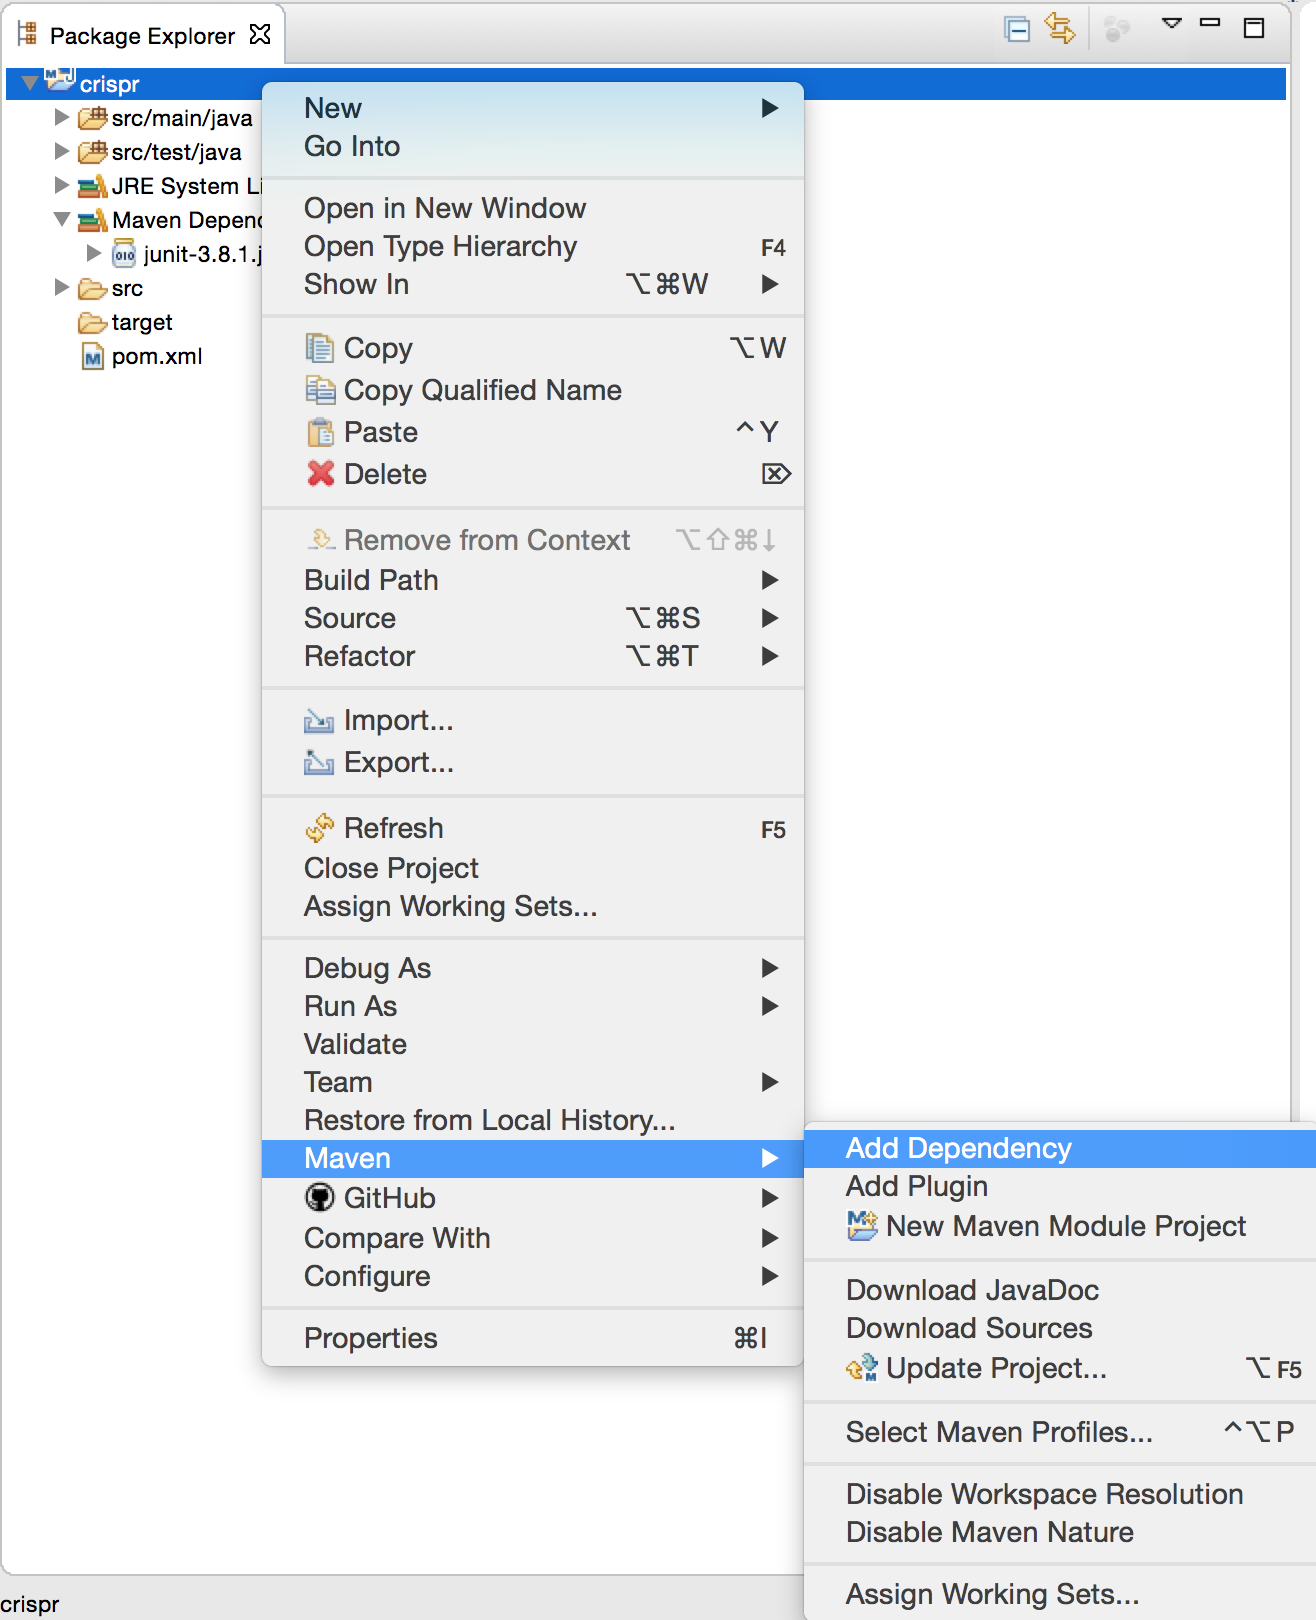
\includegraphics[width=0.55\textwidth]{figures/addMavenDependency1}
% \end{center}
In the popup window shown below, fill in the information for the {\tt libSBOLj} library. The group ID is {\bf org.sbolstandard}, and the artifact ID is {\bf libSBOLj} and the version is {\bf 2.0.0}. 
\begin{center}
  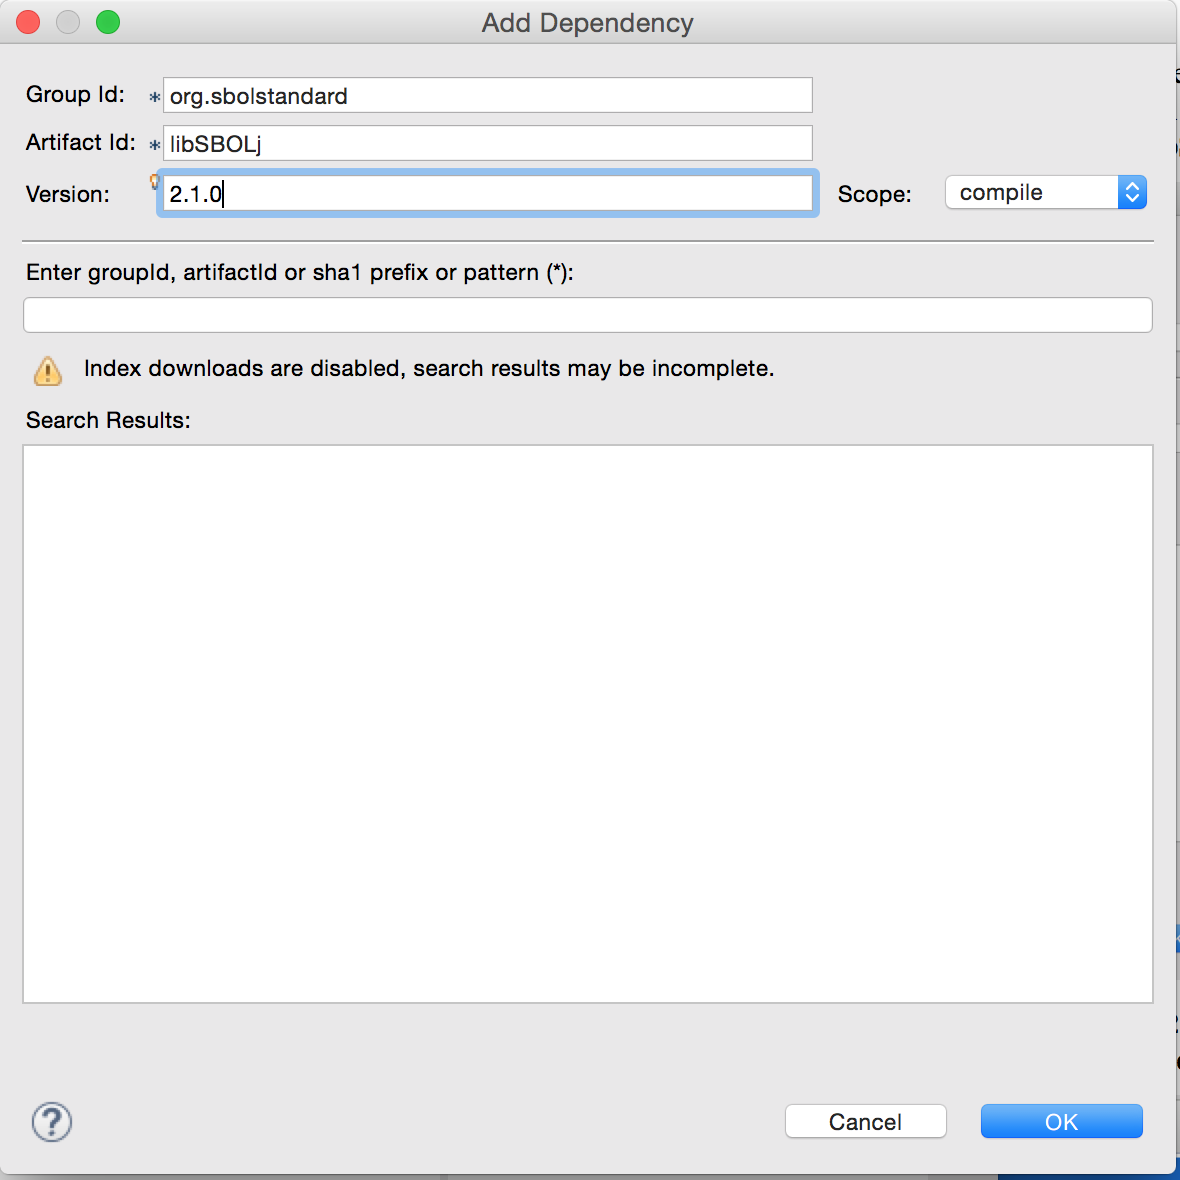
\includegraphics[width=0.55\textwidth]{figures/addMavenDependency2}
\end{center}

After this dependency is added, Maven automatically brings in the  {\tt libSBOLj-2.0.0.jar} and its dependencies from the Maven Central Repository, and places them under the {\bf Maven Dependencies} directory.
\begin{center}
  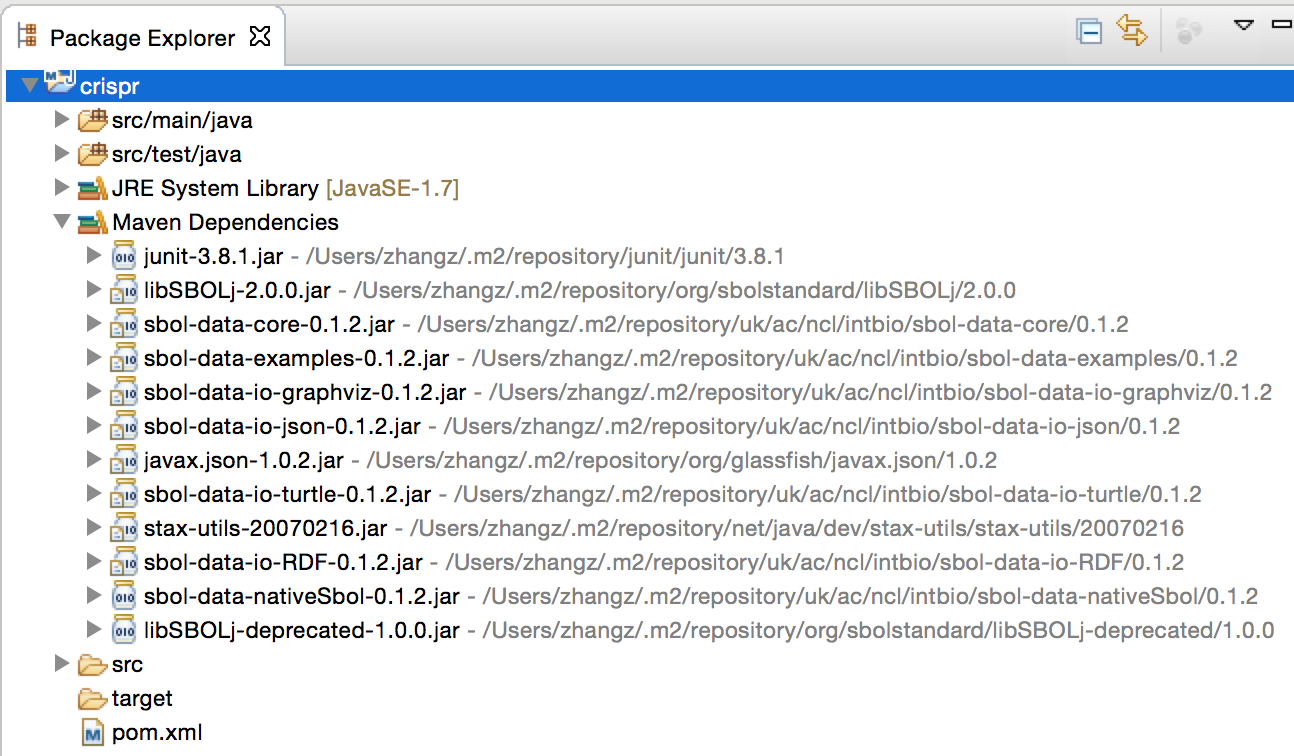
\includegraphics[width=0.8\textwidth]{figures/addMavenDependency3}
\end{center}

\section*{Add the CRISPR repression model}
Now we are ready to add the CRISPR model to our project. The model is listed as ``RepressionModel.java''  under the {\tt libSBOLj} examples directory. When the ``crispr'' project was created, two template Java class files ``App.java'' and ``AppTest.java'' were automatically created as shown below. 
\begin{center}
  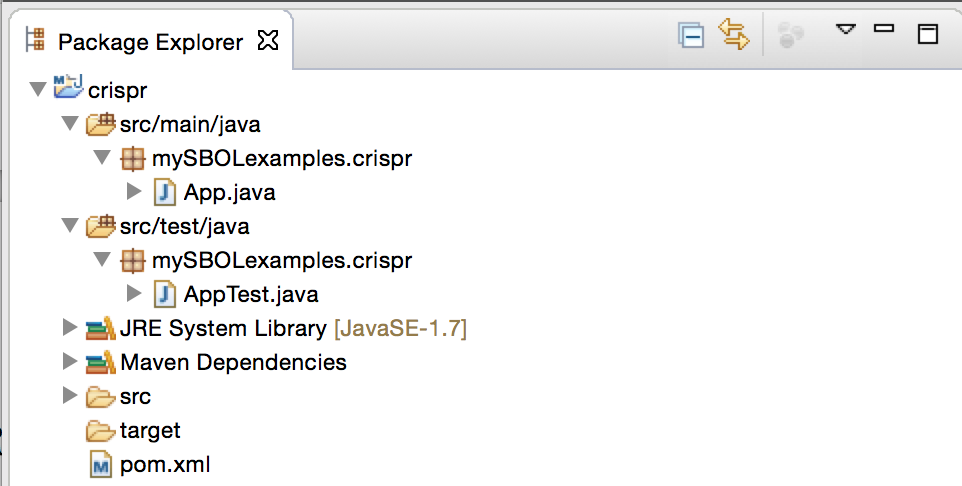
\includegraphics[width=0.8\textwidth]{figures/addCrisprModel1}
\end{center}

We can modify ``App.java'' to include the CRISPR model. First, remove all lines in ``App.java'' except the first line, which contains its package information. Then copy the full contents of ``RepressionModel.java'' except its package information to ``App.java''. Lastly, rename ``App.java'' to ``RepressionModel.java''. This file should be ready to be executed immediately, and you should be able to see the RDF/XML output in the ``console'' view. A screenshot is shown below. The ``AppTest.java'' can be modified accordingly to serve as a test file for the CRISPR repression model. 
\begin{center}
  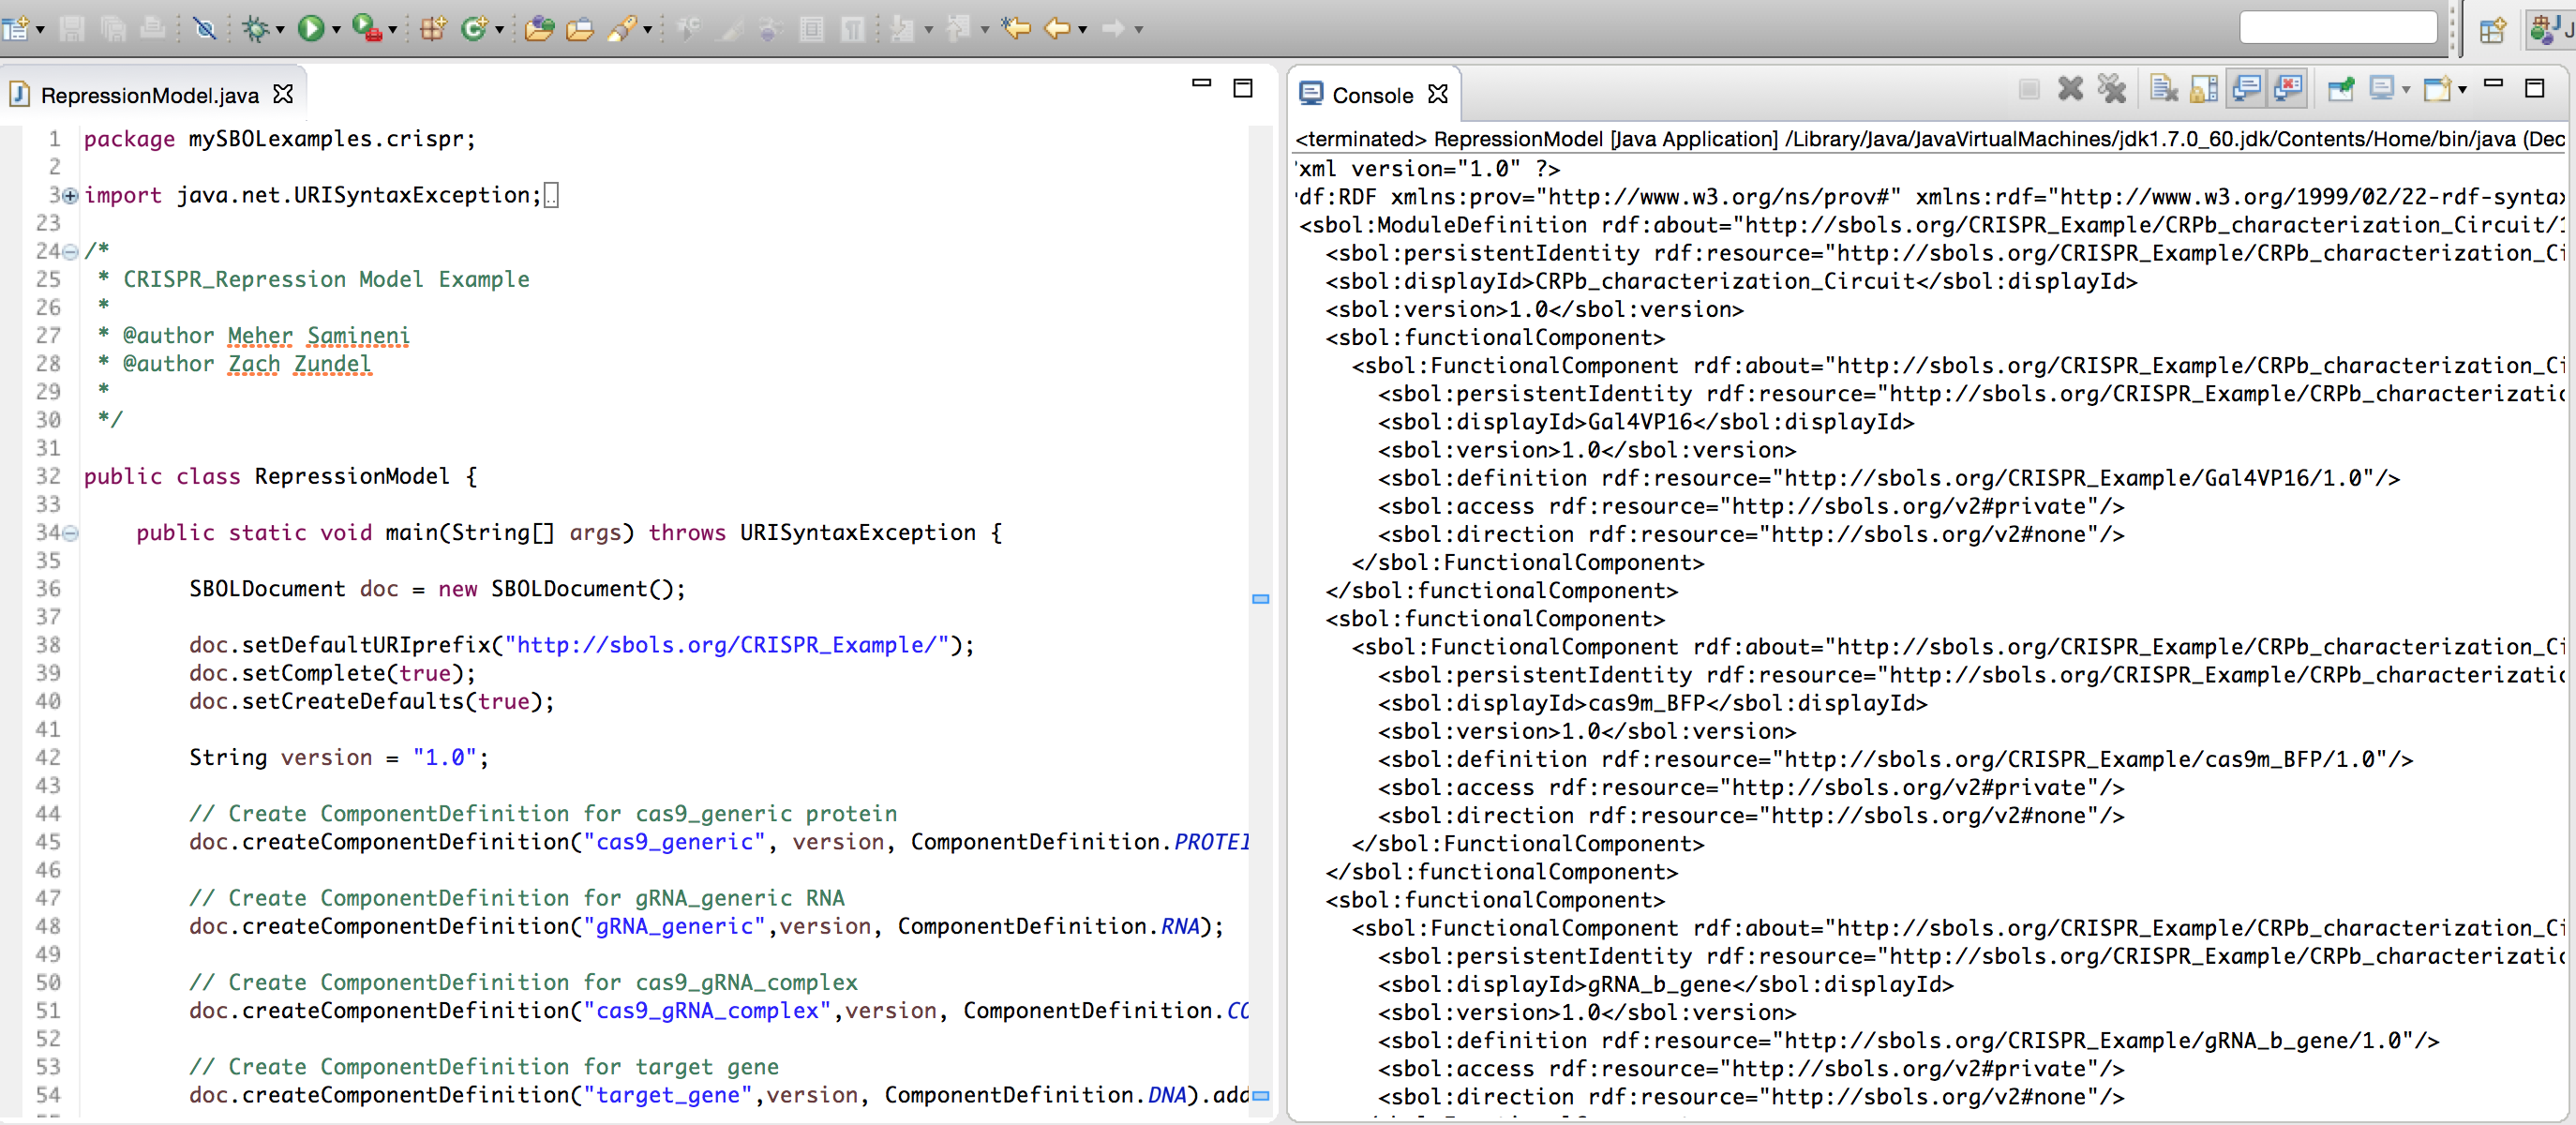
\includegraphics[width=\textwidth]{figures/addCrisprModel2}
\end{center}



\section*{Modeling CRISPR repression using {\tt libSBOLj 2.0}}
We now describe the CRISPR-based repression module and how it can be modeled and encoded using the {\tt libSBOLj 2.0} library. We use bold font in the following text and figure captions to mark available data model in SBOL 2.0. 

\subsection*{CRISPR repression model}
First, consider the CRISPR-based Repression Template \textbf{ModuleDefinition} shown in the center of Figure \ref{SBOL2}. It provides a generic description of CRISPR-based repression behavior. Namely, it includes generic \emph{Cas9}, \emph{guide RNA} (gRNA), and \emph{target} DNA \textbf{FunctionalComponent} instances. It also includes a \emph{genetic production} \textbf{Interaction} that expresses a generic target gene product.  Finally, it includes a \emph{non-covalent binding} \textbf{Interaction} that forms the Cas9/gRNA complex (shown as dashed arrows), which in turn participates in an \emph{inhibition} \textbf{Interaction} to repress the target gene product production (shown with a tee-headed arrow). The CRISPR-based Repression Template is then instantiated to test a particular CRISPR-based repression device, CRPb, by the outer CRPb Characterization Circuit \textbf{ModuleDefinition}.  This outer characterization circuit includes gene \textbf{FunctionalComponents} to produce specific products (i.e., mKate, Gal4VP16, cas9m\_BFP, gRNA\_b, and EYFP), as well as \textbf{FunctionalComponents} for the products themselves.  Next, it includes \emph{genetic production} \textbf{Interactions} connecting the genes to their products, and it has a \emph{stimulation} \textbf{Interaction} that indicates that Gal4VP16 stimulates production of EYFP.  Finally, it uses \textbf{MapsTo} objects (shown as dashed lines) to connect the generic \textbf{FunctionalComponents} in the template to the specific objects in the outer \textbf{ModuleDefinition}.  For example, the outer module indicates that the target protein is EYFP, while the cas9\_gRNA complex is cas9m\_BFP\_gRNA\_b.

\begin{figure}[tbph]
\begin{center}
  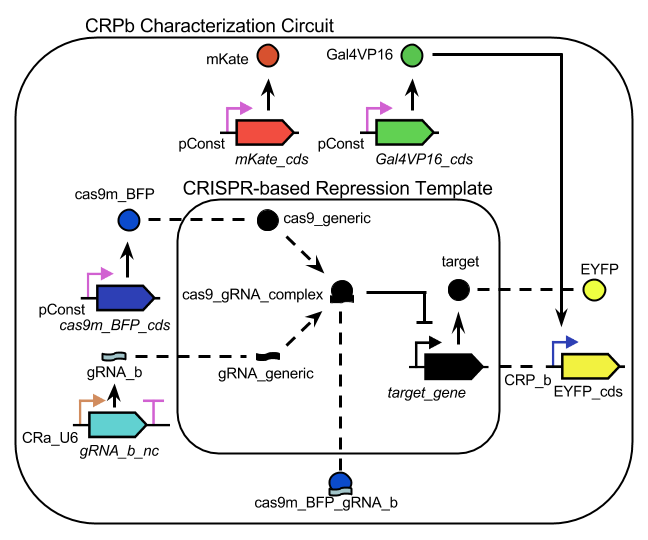
\includegraphics[width=0.95\textwidth]{figures/crispr_repression2} 
\end{center}
\caption{\label{SBOL2} Illustration of a hierarchical CRISPR-based repression module represented in SBOL 2.0 (adapted from Figure 1a in \cite{kiani2014crispr}). The CRISPR-based Repression Template \textbf{ModuleDefinition} describes a generic CRISPR repression circuit that combines a Cas9 protein with a gRNA to form a complex (represented by the dashed arrows) that represses a target gene (represented by the arrow with the tee arrowhead).  These relationships between these \textbf{FunctionalComponents} (instances of \textbf{ComponentDefinitions}) are represented in SBOL 2.0 using \textbf{Interactions}.  This \textbf{Module} is instantiated in the outer CRPb Characterization Circuit \textbf{ModuleDefinition} in order to specify the precise (including \textbf{Sequences} when provided) \textbf{FunctionalComponents}  used for each generic \textbf{FunctionalComponent}. The undirected dashed lines going into the template \textbf{Module} represent \textbf{MapsTo} objects that specify how specific \textbf{FunctionalComponents} replace the generic ones.}
\end{figure}

\subsection*{Encoding using {\tt libSBOLj 2.0}}
Program~\ref{JavaExample} illustrates the use of the {\tt libSBOLj 2.0} library using an excerpt of the Java code to express the CRISPR-based repressor design in SBOL 2.0. First, a new \textbf{SBOLDocument} is created (line 1), and is given a default URI prefix (line 2). At this point, \textbf{ComponentDefinition} and \textbf{Interaction} objects are also created for the CRISPR-based Repression Template \textbf{ModuleDefinition} (not shown).  Then, \textbf{Sequence} objects are created for those sequences provided in \cite{kiani2014crispr}.\footnote{Unfortunately, as usual, not all sequences are provided in the paper.} For example, to create the sequence for the CRP\_b promoter, we call the {\tt createSequence} method with the \emph{displayId} (CRP\_b\_seq), \emph{version} (1.0), the sequence, and the encoding used (line 3).  
Note that this method, as well as other create methods in the library, creates a \emph{compliant URI} that has the following form:
\begin{center}
http://$\langle$prefix$\rangle$/$\langle$displayId$\rangle$/$\langle$version$\rangle$
\end{center}
using the default URI prefix and provided \emph{displayId} and \emph{version}. The \emph{$\langle$prefix$\rangle$} represents a URI for a namespace (for example, {\tt www.sbols.org/CRISPR\_Example}). The author of a \textbf{TopLevel} object, such as the \textbf{Sequence} object we just created, should use a URI prefix that either they own or an organization of which they are a member owns. When using compliant URIs, the owner of a prefix must ensure that the URI of any unique \textbf{TopLevel} object that contains the prefix also contains a unique  \emph{$\langle$displayId$\rangle$} or \emph{$\langle$version$\rangle$} portion. Multiple versions of an SBOL object can exist and would have compliant URIs that contain identical prefixes and displayIds, but each of these URIs would need to end with a unique version. Lastly, the compliant URI of a non-\textbf{TopLevel} object is identical to that of its parent object, except that its displayId is inserted between its parent's displayId and version. This form of compliant URIs is chosen to be easy to read, facilitate debugging, and support a more efficient means of looking up objects and checking URI uniqueness. 

\begin{program*}[ht]
\begin{lstlisting}[language=java,style=highlight]
SBOLDocument doc = new SBOLDocument();
doc.setDefaultURIprefix("http://sbols.org/CRISPR_Example/");
doc.createSequence("CRP_b_seq", "1.0", "GCTCCGAATTTCTCGACAGATCTCATGTGAT...", !!Sequence??.<<>>IUPAC_DNA>><<); 
ComponentDefinition CRP_b = doc.createComponentDefinition("CRP_b", "1.0", !!ComponentDefinition??.<<>>DNA>><<);
CRP_b.addRole(!!SequenceOntology??.<<>>PROMOTER>><<);
CRP_b.addSequence("CRP_b_seq");
doc.createComponentDefinition("EYFP_cds", "1.0", !!ComponentDefinition??.<<>>DNA>><<).addRole(!!SequenceOntology??.<<>>CDS>><<);
ComponentDefinition EYFP_gene = doc.createComponentDefinition("EYFP_gene", "1.0", !!ComponentDefinition??.<<>>DNA>><<);
EYFP_gene.createSequenceConstraint("EYFP_gene_constraint", !!RestrictionType??.<<>>PRECEDES>><<, "CRP_b", "EYFP_cds");
doc.createComponentDefinition("Gal4VP16", "1.0", !!ComponentDefinition??.<<>>PROTEIN>><<);
ModuleDefinition CRPb_circuit = doc.createModuleDefinition("CRPb_characterization_circuit", "1.0");
Interaction EYFP_Activation = CRPb_circuit.createInteraction("EYFP_Activation", 
                                                             !!SystemsBiologyOntology??.<<>>STIMULATION>><<);
EYFP_Activation.createParticipation("GAL4VP16", "Gal4VP16").addRole(!!SystemsBiologyOntology??.<<>>STIMULATOR>><<);
EYFP_Activation.createParticipation("EYFP_gene", "EYFP_gene").addRole(!!SystemsBiologyOntology??.<<>>PROMOTER>><<);
Module Template_Module = CRPb_circuit.createModule("CRISPR_Template", "CRISPR_Template", "1.0");
Template_Module.createMapsTo("EYFP_gene_map", !!RefinementType??.<<>>USELOCAL>><<, "EYFP_gene", "target_gene");
\end{lstlisting}
\caption{\label{JavaExample}Fragments of Java code to produce part of the CRISPR Repression example using {\tt libSBOLj 2.0}.}
\end{program*}

Next, we create \textbf{ComponentDefinition} objects for each element in the module. For example, a \textbf{ComponentDefinition} of DNA type is created for the CRP\_b promoter (lines 4-6).  Note that by using compliant URIs, the sequence can be looked up using its \emph{displayId}, and since no version is provided, it is referenced by its \emph{persistentIdentity} URI (line 6). It is simply its URI without the version when using compliant URIs. The purpose of a persistent identity is to allow an object to refer to the latest version of another object using this URI. The latest version of an object is determined using \emph{semantic versioning} conventions (c.f., {\tt http://semver.org/}).

Next, we create two \textbf{ComponentDefinition} objects, one for the EYFP \emph{coding sequence} (CDS), and one for the EYFP gene (lines 7-8). We use a \textbf{SequenceConstraint} object (line 9) to indicate that the CRP\_b promoter precedes the EYFP CDS, because the sequence for the CDS has not been provided and thus cannot be given an exact \textbf{Range}. Finally, we create a protein type \textbf{ComponentDefinition} for the Gal4VP16 protein (line 10). After all the \textbf{ComponentDefinitions} are created, we create a \textbf{ModuleDefinition} object for the CRPb Characterization Circuit (line 11). 

Next, the \textbf{Interactions} between the components are specified using terms from the \emph{Systems Biology Ontology} (SBO) \cite{Courtot2011}.  One example \textbf{Interaction} is the stimulation of the \texttt{EYFP\_gene} by the Gal4VP16 protein (lines 12-14).  Now, the CRISPR-based Repression Template \textbf{Module} is instantiated and connected to the CRPb Characterization Circuit using \textbf{MapsTo} objects.  
For example, a \textbf{MapsTo} object is used to indicate that the \texttt{target\_gene} in the template should be refined to be the \texttt{EYFP\_gene} specified in the CRPb circuit (line 17).  

As we mentioned previously, the complete repression model is described in the ``RepressionModel.java'' under the libSBOLj examples directory. This example is self-contained in that you can run it to generate the RDF/XML output. Also, SBOL does not provide the specification of a mathematical model directly. It is possible, however, to generate a mathematical model using SBML~\cite{SBML} and the procedure described in~\cite{roehner2015generating}. Then, the SBOL document can reference this generated SBML model.




\bibliographystyle{ieeetr}
\bibliography{top}


\end{document}
